\chapter{A New Framework}

The development of Quantum Field Theory was driven by the need to reconcile the principles of quantum mechanics with those of special relativity. Special relativity describes the structure of spacetime and the behavior of objects moving at high velocities, while quantum mechanics governs the behavior of particles at microscopic scales. However, neither theory alone could adequately describe phenomena involving both high energies and small distances, such as particle creation and annihilation.

Quantum mechanics does not include relativistic effects:
\begin{itemize}
    \item The concept of a \textbf{limiting speed is absent}.
    \item The \textbf{energy expression} for a free particle is incompatible with the relativistic:\\
    $E_{\text{QM}} = \frac{p^2}{2m}$ instead of $E_{\text{SR}} = \sqrt{p^2c^2 + m^2c^4}$.
\end{itemize}

Special relativity, on the other hand, does not incorporate quantum principles:
\begin{itemize}
    \item It does not account for \textbf{quantization} of physical observables, first amongst all energy.
    \item The \textbf{promotion of observables to operators} acting on a Hilbert space is missing.
\end{itemize}

\begin{figure}[H]
\centering
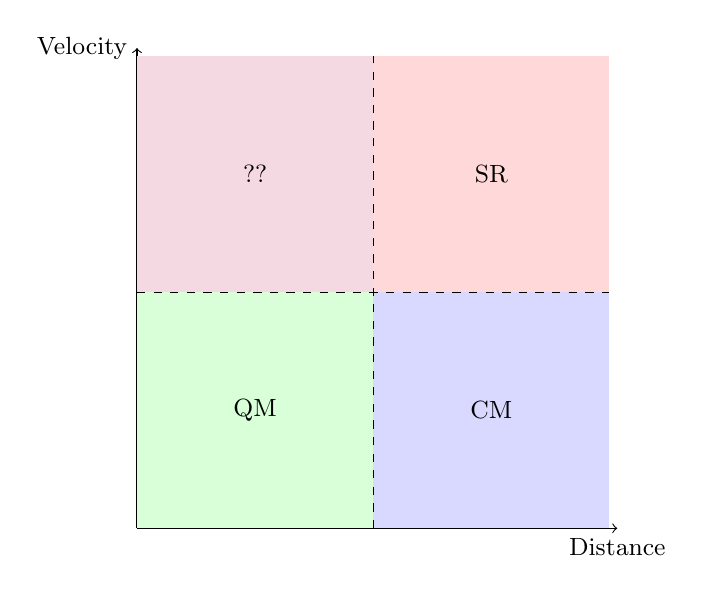
\begin{tikzpicture}[scale=1, font=\small]

\draw[->] (0,0) -- (6.1,0) node[anchor=north] {Distance};
\draw[->] (0,0) -- (0,6.1) node[anchor=east] {Velocity};

\node at (5.8,-0.3) {};
\node at (0.8,-0.3) {};
\node[rotate=90] at (-0.3,5.8) {};
\node[rotate=90] at (-0.3,0.8) {};

\fill[blue!15] (3,0) rectangle (6,3);
\node at (4.5,1.5) {CM};

\fill[green!15] (0,0) rectangle (3,3);
\node at (1.5,1.5) {QM};

\fill[red!15] (3,3) rectangle (6,6);
\node at (4.5,4.5) {SR};

\fill[purple!15] (0,3) rectangle (3,6);
\node[text=black] at (1.5,4.5) {??};

\draw[dashed] (3,0)--(3,6);
\draw[dashed] (0,3)--(6,3);

\end{tikzpicture}
\caption{Schematic diagram of the four fundamental regimes of physics.}
\end{figure}

We need a new framework to describe the regime of small distances and high velocities, where both quantum and relativistic effects are significant. The idea to overcome the shown limitations is to use expressions from SR and incorporate them into a quantum framework: a \textbf{relativistic quantum mechanics} theory.

\section{Relativistic Quantum Mechanics and its Limitations}

The first attempt to construct a relativistic quantum theory was to modify the Schrödinger equation by replacing the non-relativistic energy-momentum relation with the relativistic one. We are basically in a quantum framework:
\begin{itemize}
    \item Observables are promoted to operators acting on a Hilbert space by imposing \textit{canonical commutation relations}:\\
    $[\hat{\mathbf{x}}, \hat{\mathbf{p}}] = i\hbar \implies \hat{\mathbf{p}} = -i\hbar \frac{\mathrm{d}}{\mathrm{d}\mathbf{x}},\quad [\hat{t}, \hat{H}] = i\hbar \implies \hat{H} = i\hbar \frac{\mathrm{d}}{\mathrm{d}t}$.
    \item Operators act on a Hilbert space $\mathcal{H}$, where its states represent physical states of the system, with a \textbf{fixed number of particles}.
    \item Eigenvectors of a complete set of commuting observables form a basis for the Hilbert space; the eigenvalues correspond to the possible measurement outcomes:\\ 
    \(\hat{\mathbf{p}} \ket{p} = p \ket{p}, \quad \int \mathrm{d}p \ket{p}\bra{p} = 1\).
    \item The time evolution of states is governed by the \textbf{generalized Schrödinger equation}: $-i\hbar \frac{\partial}{\partial t} \psi(\mathbf{x}, t) = \hat{H} \psi(\mathbf{x}, t) = \sqrt{\hat{\mathbf{p}}^2c^2 + m^2c^4} \psi(\mathbf{x}, t)$ .
\end{itemize}

However, this approach leads to several issues: it cannot account for particle creation and annihilation, which are essential in relativistic contexts. Additionally, the theory struggles with maintaining causality and Lorentz invariance, and predicts an infinite number of negative energy states, leading to an unstable vacuum.

\subsection*{Production/Annihilation of Particles}

A picture in which the number of particles is fixed cannot describe processes where particles are created or destroyed, such as in high-energy collisions (LHC or other particle colliders) or in nuclear decays.

If we consider a particle with mass $m$ at rest, its energy is given by $E = mc^2$. If we now add an energy to the system, as the particle acquires momentum, its mass becomes negligible and the system is energetically favorable to create new particles. But in order to preserve physical quantities such as charge, lepton number, baryon number, etc., particles must be created in pairs.

\paragraph{Example: particle in a box.} Consider a particle of mass $m$ confined in a three-dimensional box of length $L$. The \textit{Heisenberg uncertainty principle} states that the uncertainty in position $\Delta x$ and the uncertainty in momentum $\Delta p$ satisfy the relation $\Delta x \Delta p \geq \frac{\hbar}{2}$. For a particle confined in a box, we can estimate $\Delta x \sim L$, leading to an uncertainty in momentum of at least $\Delta p \sim \frac{2\hbar}{L}$. If we take the particle to the ultrarelativistic regime,\footnote{In the ultrarelativistic regime, the particle's kinetic energy is much greater than its rest mass energy: \(E^2 = p^2c^2 + m^2c^4 \approx p^2c^2\).} its energy can be approximated as \(E \approx pc\). Therefore, the uncertainty in energy will be:
\[
    \Delta E \geq \frac{2\hbar c}{L}.
\]
If we want to avoid the production of particle-antiparticle pairs, we must ensure that the energy uncertainty is less than the energy required to create such a pair, which is \(2mc^2\). But if we decrease the size of the box \(L\) to increase the precision in position, we increase the uncertainty in energy.
\[
    2mc^2 = \frac{2\hbar c}{L} \implies L = \frac{\hbar}{mc} = \lambda_c.
\]
Here, \(\lambda_c\) is the Compton wavelength of the particle, representing a fundamental limit to the precision with which we can localize a particle without inducing pair production. If we try to confine the particle within a region smaller than its Compton wavelength, the energy uncertainty becomes sufficient to create particle-antiparticle pairs, making it impossible to describe the system with a fixed number of particles.

We need a framework that allows for a variable number of particles, accommodating the creation and annihilation processes inherent in relativistic quantum phenomena (as we will see, a Fock space formalism is required: \(\mathcal{F} = \bigoplus_{n} \mathcal{H}_n\)).

\subsection*{Violation of Causality}
